\documentclass[12pt, titlepage]{article}
\usepackage[letterpaper, margin=2.5cm]{geometry}
\usepackage[utf8]{inputenc}
\usepackage{float}
\usepackage{graphicx}
\usepackage[spanish]{babel}
\usepackage{url}

%opening
\title{Procesos naturales que utilizan memoria}
\author{Barrera Pérez Carlos Tonatihu \\ Profesor: Genaro Juárez Martínez \\ Computing Selected Topics \\ Grupo: 3CM8 }

\begin{document}

\maketitle

\newpage
\section{Colonia de hormigas}
Las hormigas trabajan en conjunto para encontrar caminos entre fuentes de alimento y su hormiguero, las hormigas son ciegas por lo utilizan señales químicas (feromonas) que ellas mismas producen y son dejadas en el suelo para poder orientarse y recordar el camino que deben de seguir para no perderse.

Es aquí en donde entra el uso de memoria ya que se debe de recordar los caminos que trazan las hormigas en su recorrido ya que no siguen siempre el mismo camino desde un punto A a un punto B, puede ser que las hormigas utilicen diferentes rutas entre estos dos puntos por lo que se debe tener un registro de los caminos que utilizan con el objetivo de determinar cual es el camino más corto entre dos puntos. A continuación se explica más a fondo este proceso \cite{HORMIGA}.

\begin{enumerate}
    \item Una hormiga se mueve alrededor de la colonia.
    \item Si esta encuentra comida, retorna a la colonia de manera más o menos directa, dejando un rastro de feromonas.
    \item Estas feromonas son atractivas, las hormigas más cercanas  se verán atraídas por ellas y seguirán su pista de manera más o menos directa (lo que quiere decir que a veces pueden dejar el rastro), que les lleva a la fuente de comida encontrada por la exploradora.
    \item Al regresar a la colonia con alimentos estas hormigas depositan más feromonas, por lo que fortalecen las rutas de conexión.
    \item Si existen dos rutas para llegar a la misma fuente de alimentos, en una misma cantidad de tiempo, la ruta más corta será recorrida por más hormigas que la ruta más larga.
    \item En consecuencia, la ruta más corta aumentará en mayor proporción la cantidad de feromonas depositadas y será más atractiva para las siguientes hormigas.
    \item La ruta más larga irá desapareciendo debido a que las feromonas son volátiles.
    \item Finalmente, todas las hormigas habrán determinado y escogido el camino más corto.
\end{enumerate}

\begin{figure}[H]
    \begin{center}
        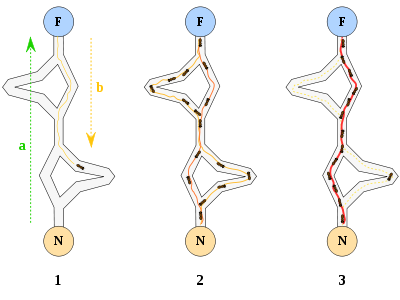
\includegraphics[width=6cm, height=5cm]{./img/ants.png}
        \caption{Representación grafica de una colonia de hormigas}
        \label{fig:ants}
    \end{center}
\end{figure}

El análisis de este comportamiento es importante ya que permite ser utilizado para resolver problemas de optimización de rutas, evaluando muchos caminos pero sin utilizar demasiada memoria ya que estos caminos se van descartando como se planteo en el proceso descrito con anterioridad.
\section{Procesos genéticos}
En la naturaleza los individuos de una población compiten entre si en la búsqueda de recursos tales como comida, agua y refugio o incluso de un compañero. Aquellos individuos que tienen más éxito en sobrevivir y en atraer compañeros tienen mayor probabilidad de generar un gran número de descendientes. Por lo que los genes más adaptados se propagarán en sucesivas generaciones. La combinación de individuos de buenas características pueden producir descendientes que sean superindividuos y con eso se logra la evolución a seres con mejores características \cite{GEN}.

\begin{figure}[H]
    \begin{center}
        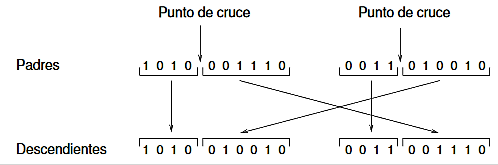
\includegraphics[width=8cm, height=3cm]{./img/geneticos.png}
        \caption{Ejemplo de un cruce en una población}
        \label{fig:geneticos}
    \end{center}
\end{figure}

El uso de memoria es fundamental en este proceso ya que se necesita guardar poblaciones que son las que a lo largo de muchas generaciones pueden mutar o cruzarse con otras poblaciones, así que es necesario el guardar toda esta información.
\section{Neuronas}
Las neuronas se interconectan entre sí de forma paralela, y no formando un circuito cerrado como el sistema sanguíneo. De alguna forma, una neurona es un procesador de información muy simple:

\begin{enumerate}
    \item Canal de entrada: dendritas.
    \item Procesador: soma.
    \item Canal de salida: axón.
\end{enumerate}

Una neurona cerebral puede recibir unas 10.000 entradas y enviar a su vez su salida a varios cientos de neuronas. La conexión entre neuronas se llama sinapsis. No es una conexión física, si no que hay unos 2 mm de separación. Son conexiones unidireccionales, en la que la transmisión de la información se hace de forma eléctrica en el interior de la neurona y de forma química entre neuronas; gracias a unas sustancias específicas llamadas neurotransmisores.

\begin{figure}[H]
    \begin{center}
        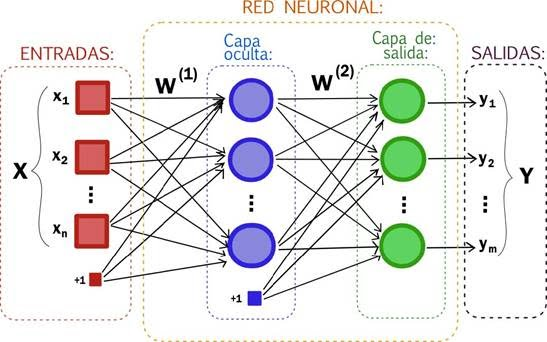
\includegraphics[width=12cm, height=6cm]{./img/red.jpg}
        \caption{Representación gráfica de una red neuronal artificial y sus componentes}
        \label{fig:red}
    \end{center}
\end{figure}

Este comportamiento se puede representar de forma matemática para ser implementado en redes neuronales artificiales en las cuales cada neurona está conectada con otras a través de unos enlaces. En estos enlaces el valor de salida de la neurona anterior es multiplicado por un valor de peso. Estos pesos en los enlaces pueden incrementar o inhibir el estado de activación de las neuronas adyacentes. Del mismo modo, a la salida de la neurona, puede existir una función limitadora o umbral, que modifica el valor resultado o impone un límite que se debe sobrepasar antes de propagarse a otra neurona. Esta función se conoce como función de activación.

Estos sistemas aprenden y se forman a sí mismos, en lugar de ser programados de forma explícita, y sobresalen en áreas donde la detección de soluciones o características es difícil de expresar con la programación convencional. Para realizar este aprendizaje automático, normalmente, se intenta minimizar una función de pérdida que evalúa la red en su total. Los valores de los pesos de las neuronas se van actualizando buscando reducir el valor de la función de pérdida. Este proceso se realiza mediante la propagación hacia atrás. 
\section{Enjambres}
La inteligencia de enjambre es el comportamiento colectivo de sistemas descentralizados y auto-organizados, naturales o artificiales. Inspirados por la naturaleza, especialmente por ciertos sistemas biológicos, los sistemas de inteligencia de enjambre están típicamente formados por una población de agentes simples que interactúan localmente entre ellos y con su medio ambiente. Los agentes siguen reglas simples y, aunque no existe una estructura de control centralizado que dictamine el comportamiento de cada uno de ellos, las interacciones locales entre los agentes conduce a la emergencia de un comportamiento global complejo.
\begin{figure}[H]
    \begin{center}
        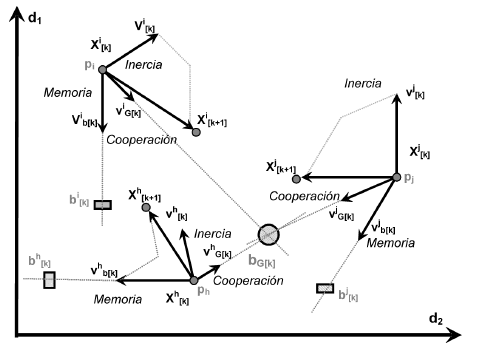
\includegraphics[width=6cm, height=5cm]{./img/particula.png}
        \caption{Comportamiento de partículas}
        \label{fig:particula}
    \end{center}
\end{figure}
Un ejemplo de esto son los enjambres de particulas en los cuales cada partícula (individuo) tiene una posición, $\overrightarrow{p}$ (que en 2 dimensiones vendrá determinado por un vector de la forma (x,y)), en el espacio de búsqueda y una velocidad, $\overrightarrow{v}$ (que en 2 dimensiones vendrá determinado por un vector de la forma $(v_x,v_y)$), con la que se mueve a través del espacio. Además, como partículas de un mundo real físico, tienen una cantidad de inercia, que los mantiene en la misma dirección en la que se movían, así como una aceleración (cambio de velocidad), que depende principalmente de dos características:

\begin{enumerate}
    \item Cada partícula es atraída hacia la mejor localización que ella, personalmente, ha encontrado en su historia (mejor personal).
    \item Cada partícula es atraída hacia la mejor localización que ha sido encontrada por el conjunto de partículas en el espacio de búsqueda (mejor global).
\end{enumerate}

La fuerza con que las partículas son empujadas en cada una de estas direcciones depende de dos parámetros  que pueden ajustarse (atracción-al-mejor-personal y atracción-al-mejor-global), de forma que a medida que las partículas se alejan de estas localizaciones mejores, la fuerza de atracción es mayor. También se suele incluir un factor aleatorio que influye en cómo las partículas son empujadas hacia estas localizaciones \cite{PARTICULA}.
\section{Fractales}
Fractales naturales son objetos naturales que se pueden representar con muy buena aproximación mediante fractales matemáticos con autosimilaridad estadística. Los fractales encontrados en la naturaleza se diferencian de los fractales matemáticos en que los naturales son aproximados o estadísticos y su autosimilaridad se extiende solo a un rango de escalas (por ejemplo, a escala cercana a la atómica su estructura difiere de la estructura macroscópica).

Un fractal natural es un elemento de la naturaleza que puede ser descrito mediante la geometría fractal. Las nubes, las montañas, el sistema circulatorio, las líneas costeras o los copos de nieve son fractales naturales. Esta representación es aproximada, pues las propiedades atribuidas a los objetos fractales ideales, como el detalle infinito, tienen límites en el mundo natural \cite{FRACTAL}. 
\begin{figure}[H]
    \begin{center}
        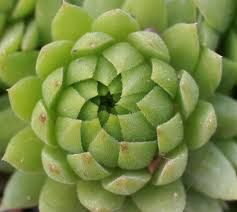
\includegraphics[width=6cm, height=5cm]{./img/fractal.jpg}
        \caption{Ejemplo de un fractal en la naturaleza}
        \label{fig:fractales}
    \end{center}
\end{figure}
Una forma de producir fractales es mediante algoritmos recursivos y es aquí en donde entra en juego la memoria ya que al trabajar con recurrencia se trabaja con una pila la cual utiliza memoria para saber en que punto del proceso se encuentra el algoritmo y en que momento termina la recurrencia.
\bibliography{reporte} 
\bibliographystyle{ieeetr}

\end{document}
